% Generic College Assignment Template
\documentclass[12pt,a4paper]{article}

% Package imports
\usepackage[utf8]{inputenc}
\usepackage[margin=2.5cm]{geometry}
\usepackage{amsmath,amssymb,amsthm}
\usepackage{graphicx}
\usepackage{hyperref}
\usepackage{enumitem}
\usepackage{fancyhdr}
\usepackage{cite}
\usepackage{listings}
\usepackage{xcolor}
\usepackage{float}

% Header and footer setup
\pagestyle{fancy}
\fancyhf{}
\lhead{\courseName}
\rhead{\authorName}
\cfoot{\thepage}

% Code listing settings (optional, for programming assignments)
\lstset{
    basicstyle=\ttfamily\small,
    breaklines=true,
    frame=single,
    numbers=left,
    numberstyle=\tiny,
    commentstyle=\color{gray},
    keywordstyle=\color{blue}
}

% Document metadata
\newcommand{\authorName}{Sam Freund}
\newcommand{\courseName}{Math 2480}
\newcommand{\assignmentTitle}{Activity 1}
\newcommand{\dueDate}{\today}

% Theorem environments (uncomment if needed)
% \newtheorem{theorem}{Theorem}
% \newtheorem{lemma}{Lemma}
% \newtheorem{definition}{Definition}

\renewcommand{\thesubsection}{\thesection.\alph{subsection}}

\begin{document}

% Title section
\begin{center}
    {\Large \textbf{\assignmentTitle}}\\[0.5em]
    {\large \courseName}\\[1em]
    \authorName\ \\
    Date: \dueDate
\end{center}

\vspace{1em}
\hrule
\vspace{2em}

% Main content starts here
\section{Part 1: Summarizing One Categorical Variable}

\subsection{Frequency Table}

\begin{tabular}{|c|l|c|c|}
\hline
Color & Frequency & Relative Frequency \\
\hline
BLACK & 44 & 0.13622291 \\
BLUE & 37 & 0.11455108 \\
GOLD & 40 & 0.12383901 \\
GRAY & 47 & 0.14551084 \\
GREEN & 21 & 0.06501548 \\
RED & 15 & 0.04643963 \\
SILVER & 74 & 0.22910217 \\
WHITE & 45 & 0.13931889 \\
\hline
\end{tabular}

\subsection{Appropriate Plot for Summary of Color}

An appropriate plot for summarizing a categorical variable like color is a bar chart. 
Each bar represents a different color, and the height of the bar corresponds to the 
frequency or relative frequency of that color in the dataset.

\pagebreak

\subsection{Bar Chart of Color Counts}

\begin{figure}[H]
    \centering
    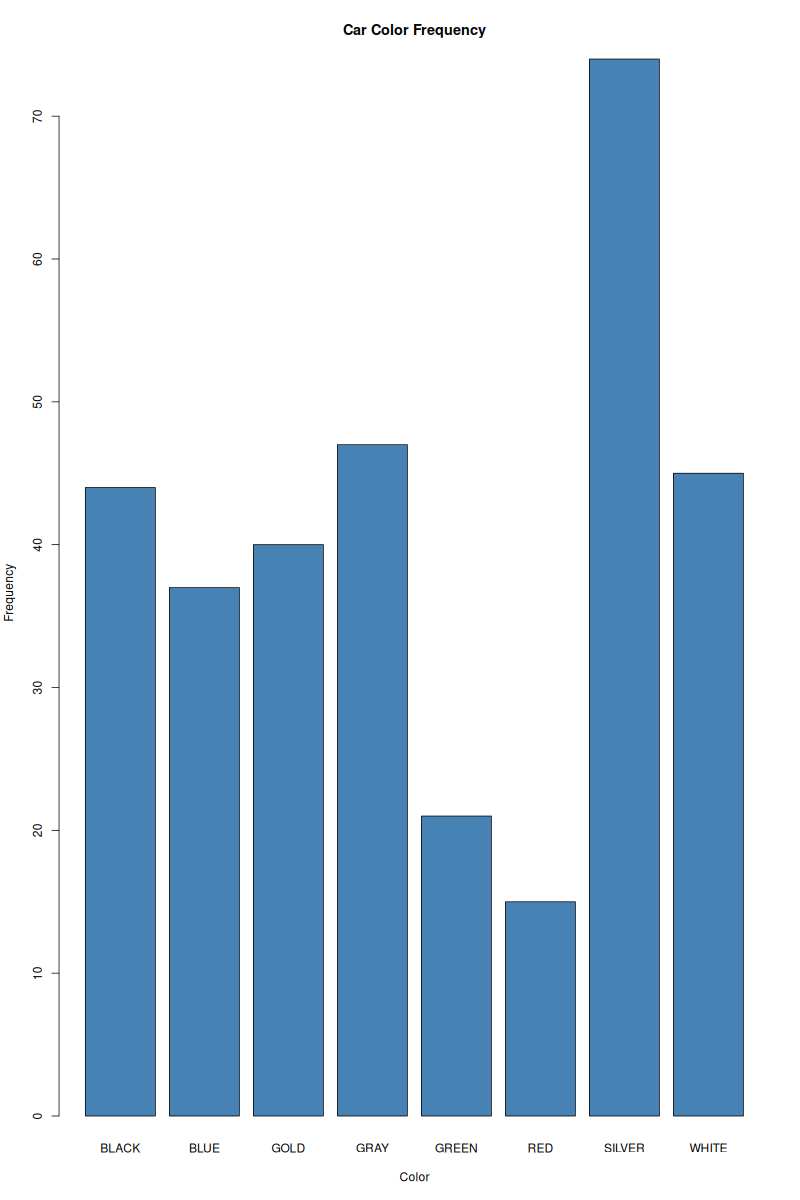
\includegraphics[width=0.8\textwidth]{colorBarChart.png}
    \caption{Bar Chart of Color Counts}
    \label{fig:color_bar_chart}
\end{figure}

\newpage

\section{Summarizing One Quantitative Variable}

\subsection{Mean and Variance}

\begin{tabular}{|c|c|}
\hline
Mean & 11754.1 \\
Variance & 7648459 \\
\hline
\end{tabular}

\subsection{Five Number Summary}

\begin{tabular}{|c|c|}
\hline
Minimum & 5995 \\
First Quartile (Q1) & 9967.5 \\
Median (Q2) & 11000 \\
Third Quartile (Q3) & 14500 \\
Maximum & 20995 \\
\hline
\end{tabular}

\subsection{Boxplot of Price}

The outlier in this dataset is located at \$20,995.

\begin{figure}[H]
    \centering
    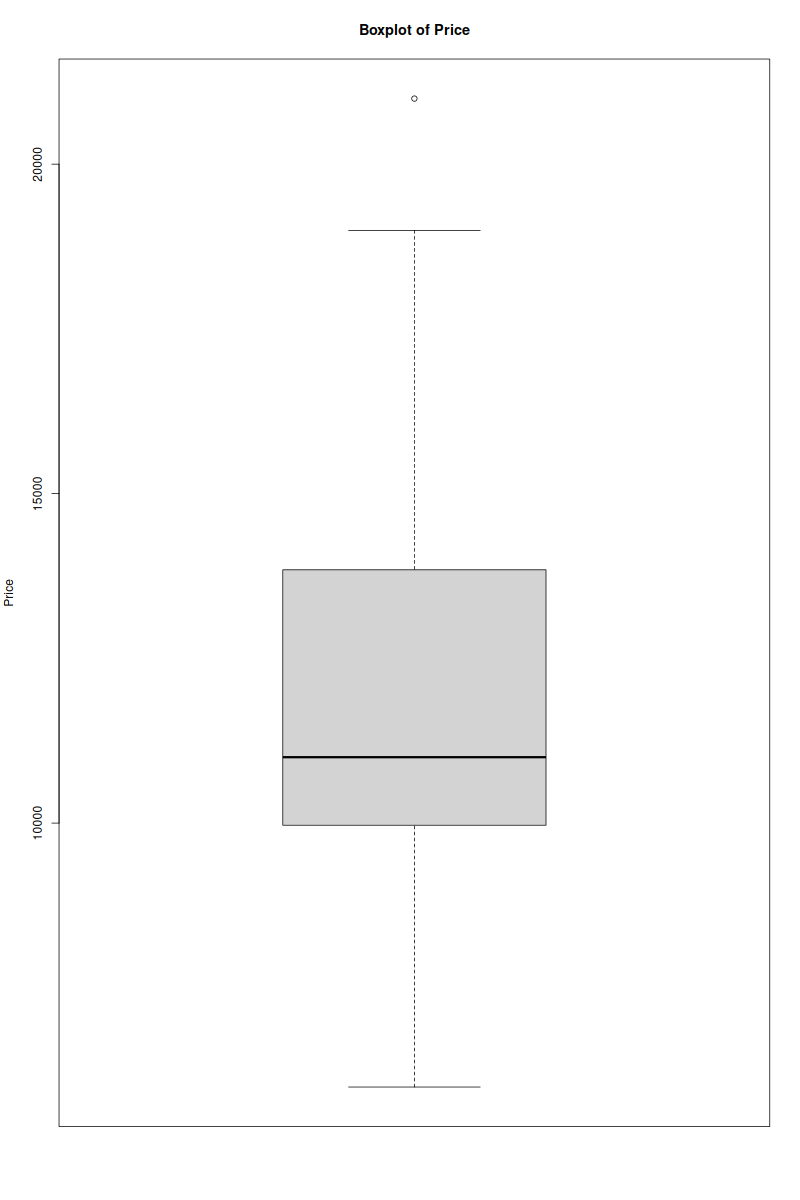
\includegraphics[width=0.6\textwidth]{boxPlot.png}
    \caption{Boxplot of Price}
    \label{fig:price_boxplot}
\end{figure}

\stepcounter{subsection}

\subsection{Log Transformation of Price Boxplot}

New outlier of $8.698681$.

\begin{figure}[H]
    \centering
    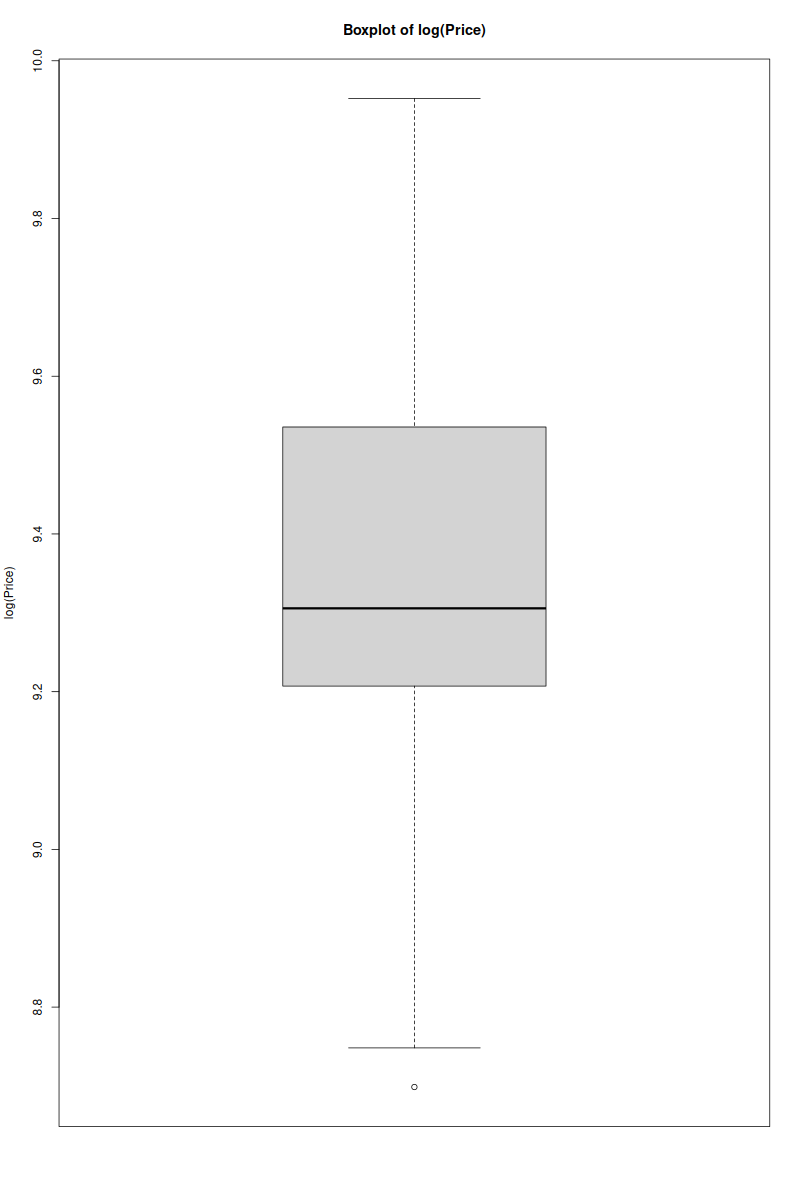
\includegraphics[width=0.6\textwidth]{logBoxplot.png}
    \caption{Boxplot of Log-Transformed Price}
    \label{fig:log_price_boxplot}
\end{figure}

\subsection{Normal and Log Price Histograms}

\begin{figure}[H]
    \centering
    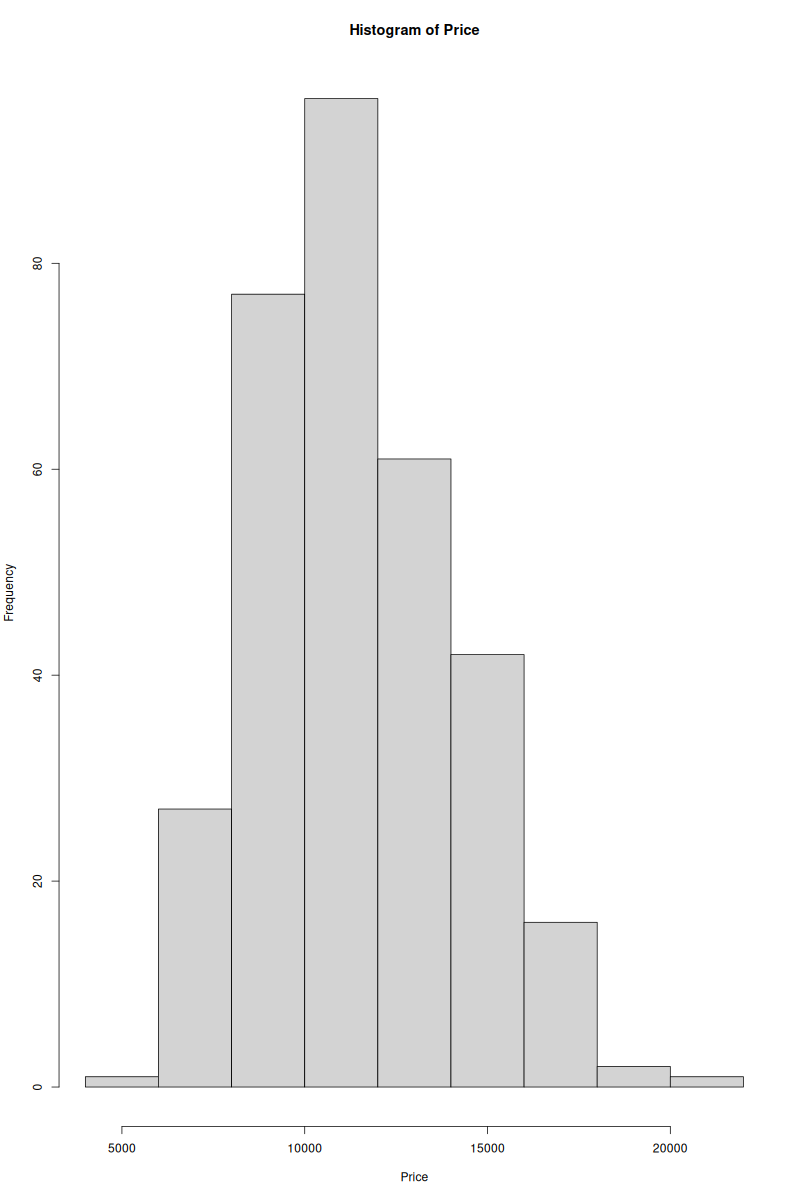
\includegraphics[width=0.45\textwidth]{priceHistogram.png}
    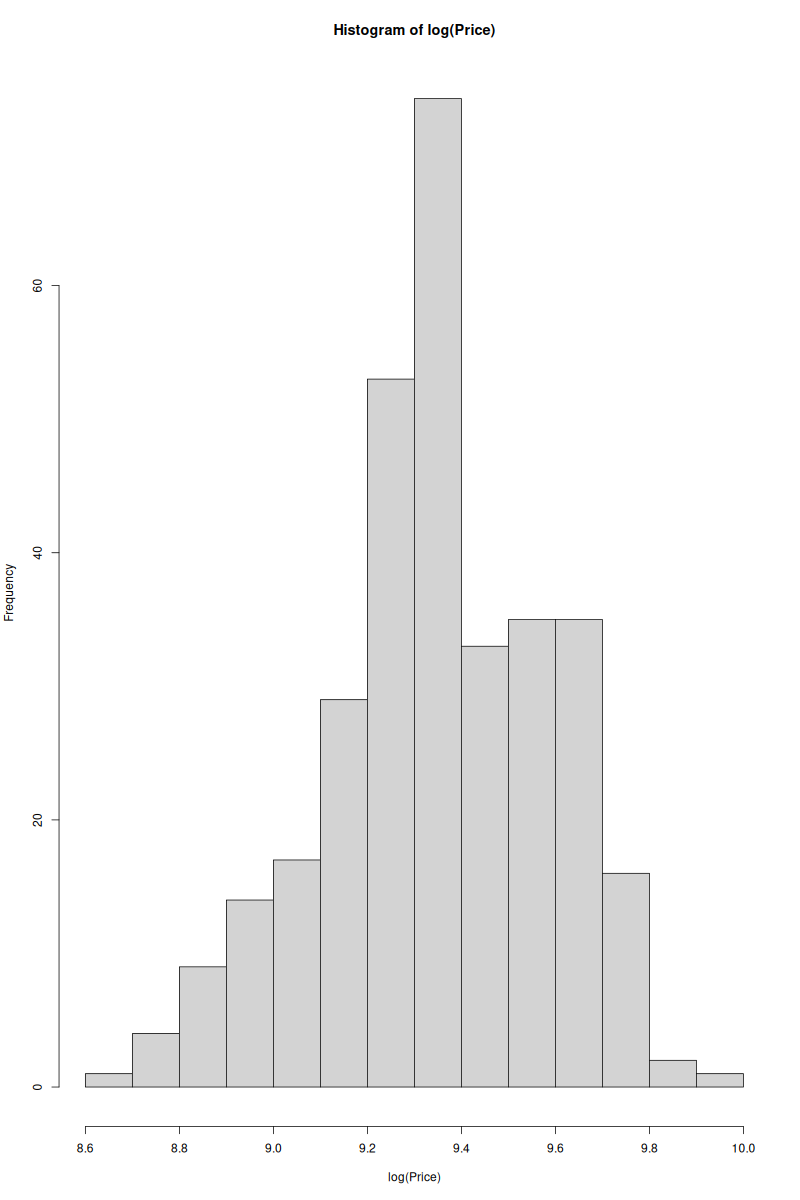
\includegraphics[width=0.45\textwidth]{logPriceHistogram.png}
    \caption{Histograms of Normal Price (left) and Log-Transformed Price (right)}
    \label{fig:price_histograms}
\end{figure}

The normal histogram (Figure \ref{fig:price_histograms}, left) appears right-skewed, while 
the log-transformed histogram (Figure \ref{fig:price_histograms}, right) appears more 
symmetric although somewhat left-skewed.

\subsection{Five Number Summary Without Outliers}

\begin{tabular}{|l|c|c|}
\hline
 & Original Price & Log-Transformed Price \\
\hline
Minimum & 5995 & 5995.0 \\
First Quartile (Q1) & 9967.5 & 9950.0 \\
Median (Q2) & 11000 & 10999.5 \\
Third Quartile (Q3) & 14500 & 13800.0 \\
Maximum & 20995 & 18995.0 \\
\hline
\end{tabular}

\vspace{1em}

We see that the minimum remains the same, as no outliers were removed on the lower end. Conversely, 
our maximum decreased significantly after removing the upper outlier, indicating that the highest 
price was indeed an outlier. We see our first and third quartiles, along with the median, also decrease, 
reflecting the overall shift in the distribution after outlier removal.

\newpage

\section{Code Appendix}

\lstinputlisting[language=R, caption=R Code for Lab 1]{lab1.R}

\end{document}
